\documentclass{standalone}
\usepackage{tikz}

\begin{document}
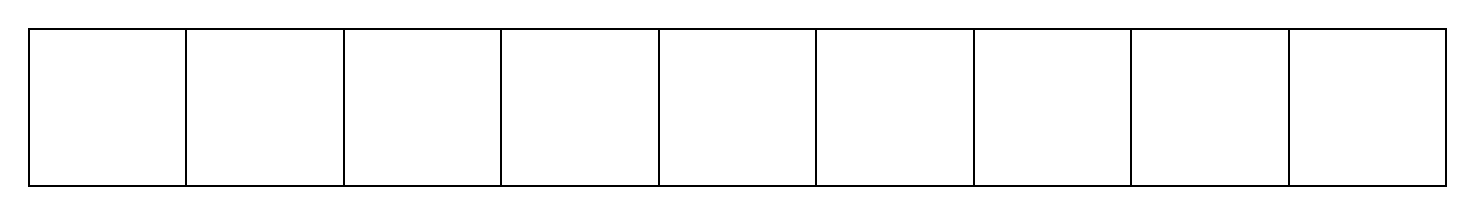
\begin{tikzpicture}[scale=2]
    % Define the first diamond pattern
    \foreach \i in {1,3,5} {
        \draw[thick] (\i,0) -- ++(0,1) -- ++(-1,0) -- ++(0,-1) -- cycle;
    }

    % Define the second diamond pattern
    \foreach \i in {4,6,8} {
        \draw[thick] (\i,0) -- ++(0,1) -- ++(-1,0) -- ++(0,-1) -- cycle;
    }

    % Define the third diamond pattern
    \foreach \i in {2,7,9} {
        \draw[thick] (\i,0) -- ++(0,1) -- ++(-1,0) -- ++(0,-1) -- cycle;
    }
\end{tikzpicture}
\end{document}